\section{Importance Sampling Technique}
    Importance sampling's main concept is that some random input variables' (or vectors') values have a more profound influence on the estimated quantity than others. The estimator's variance can be reduced if these "important" values are sampled more frequently, i.e., from a biased density function. The simulation results are then weighted to remove the bias caused by sampling from the skewed density function.\\
    The important sampling techniques consist of two main steps:
    The first is an alteration to the original input procedure. To give some "important" parts of the sample space more samples, samples are drawn from another probability density function (PDF), known as an \textit{importance density function}. The selection of the biased importance density function is the critical challenge in putting the importance sampling approaches into practice. The other involves eliminating the distortion by averaging the results of various samples (realizations) using weights associated with the distortion, preserving the estimated quantity's actual mean in the process.
    
    \subsection{Mathematical Expression of Importance Sampling Technique}
        Let $x$ denote a random variable (or vector) with a (joint) pdf of $p(x)$. The objective is to derive the moments (mean and variance) of the function $h=f(x)$, where $f$ is a specified, deterministic function (operator). 
        The mean and variance of $h$ can be written as:
        $$\mu_h=E[h]=E[f(x)]=\int_\Omega f(x)p(x)dx$$
        $$\sigma_h^2=E{[f(x)-\mu_h]^2}=\int_\Omega[f(x)-\mu_h]^2 p(x)dx = \int_\Omega f^2(x)p(x)dx-\mu^2_h$$
        Where, $\Omega$ is a probability space, $E$ represents statistical expectation and $\mu_h$ and $\sigma_h^2$ are the mean and variance of $h=f(x)$, respectively. \\ 
        The two integrals mentioned above can be solved in two ways: either by analytical methods, which result in an exact solution, or approximation methods (such as the Monte Carlo), which give an estimation of the real solution. 
        To estimate the $\mu_h$ using the Monte Carlo (MC) method, samples $(x_i, i=1,2,…,N)$ will be randomly generated from the density function $p(x)$ and the sample mean $(\mu_{MC})$ and the variance of the samples $(\sigma_{MC}^2)$ will be calculated as follow:
        $$\mu_{MC}=\frac{1}{N}\sum_{i=1}^{N} f(x_i)$$
        $$\sigma_{MC}^2=\frac{1}{N}\sum_{i=1}^{N}f^2(x_i)-(\frac{1}{N}\sum_{i=1}^{N} f(x_i))^2$$
        Where $\mu_{MC}$ and $\sigma_{MC}^2$ are the mean and variance of $h=f(x)$ estimated using crude MC simulation method, respectively.\\ 
        As the number of samples increases, it is preferable to employ some technique that reduces the estimation variance more quickly. One such method that lowers estimation variance and, as a result, lowers statistical error considerably more rapidly than MC procedures is the importance sampling technique.
        The main idea behind importance sampling is to focus on and take samples $x$ in areas where the value of the function $f(x)$ significantly impacts the estimated quantity instead of focusing on areas where the impact is minor. This process's bias (or distortion) must be removed by weighing the sample values appropriately.
        Suppose we sample $x_i  ,i=1,2,…,N$, from an importance density function $q(x)$ rather than the original density function $p(x)$, where $q(x)$ is zero only if $p(x)$ is zero. To preserve the mean (i.e., to correct the bias), the original function $f(x)$ should be modified. A modified function $f_q(x)$ is defined as:
        $$f_q(x)=f(x) w(x)$$
        Where $w(x)=p(x)/q(x)$ is called a weight function. 
        The mean and variance of f(x) can also be written as:
        $$\mu_{IS}=\frac{1}{N} \sum_{i=1}^{N}f(x_i)w(x_i)$$
        $$\sigma_{IS}^2=\frac{1}{N} \sum_{i=1}^N f^2(x_i)w(x_i)-\mu_{IS}^2$$
        Where $\mu_{IS}$ and $\sigma_{IS}^2$ are the mean and variance of $h=f(x)$ estimated using the IS-MC simulation method, respectively. 
        
    \subsection{Selection of Importance Density Functions}
        While importance sampling estimates may have a significantly lower variance than their MC counterparts, choosing an appropriate importance density function is a difficult process that is hard to generalize and has served as the inspiration for numerous papers in the statistics and simulation literature. \\
        The importance density function $q(x)$ should be chosen in a way that minimizes the estimated variance quantity $\sigma_{IS}^2$ and lowers computational effort in estimating mean quantity $\mu_{IS}$. However, it is difficult to minimize the variance of IS estimation directly as a function of an unknown density function $q(x)$. There are several available techniques to estimate the importance density function. Some of them involve a manual trial and error process in which $q(x)$ is chosen from the same family distribution of the original distribution $p(x)$ but with different parameters. Some examples are: (a) \textit{Variance Scaling} (VS) and (b) \textit{Mean Translation} (MT), or (c) their combination \cite{lu_improved_1988}. \\
        The concepts of MT, VS, and their combination are illustrated in Fig.~\ref{fig:IS_techniques}, where $p(x)$ is the original density function, $q(x)$ is the proposed importance density function, and f(x) is a function of the model under study. 
        
            \begin{figure}[H]
        \centering
        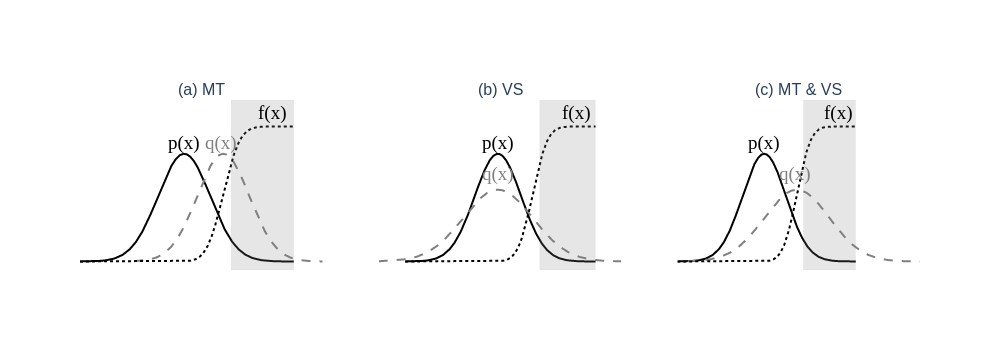
\includegraphics[scale=0.40]{Figures/Images/Importance Sampling Technique/IS_techniques.png}
        \caption{Schematic diagrams showing (a) MT, (b) VS, and (c) their combination in one dimension. The shaded area indicates the effective IS probability density. \protect\cite{lu_improved_1988}}
        \label{fig:IS_techniques}
    \end{figure}
        
        As can be seen in Fig.~\ref{fig:IS_techniques}, samples with associated high $f(x)$ are located in the tail region of $p(x)$ with a very low probability of occurrence (gray shaded area). In this situation, generating more important samples more frequently is preferable. That's why in MT, the $q(x)$ is the same probability distribution function as the $p(x)$ but with the shifted mean value towards the more consequential area, which is illustrated in Fig.~\ref{fig:IS_techniques}-a. Another way to enlarge the sampling frequency is to increase the variance of the $p(x)$ to generate more samples in the tale region of the $p(x)$. This is the logic behind VS technique that can be seen in Fig.~\ref{fig:IS_techniques}-b. The combination of MT and VS is also shown in Fig.~\ref{fig:IS_techniques}-c.
    	
    \subsection{Markov Chain Monte Carlo Importance Sampling (MCMC-IS) Technique} 
        The manual trial and error process to estimate the importance density function can be very time-consuming as finding the optimal importance density parameters may require solving the problem many times. Other methods have been proposed to estimate the near-optimal importance sampling distribution more systematically. One of these methods is called Markov Chain Monte Carlo Importance Sampling (MCMC-IS), which is proposed by \cite{parpas_importance_2015}.\\
        The MCMC-IS framework consists of three steps: (1) generate samples from the zero-variance distribution using an MCMC algorithm, (2) construct an approximate zero-variance distribution using a KDE \textit{(Kernel Density Estimation)} algorithm, and (3) sample from the approximate zero-variance distribution to form a lower-variance importance sampling estimate.\\
        \textit{Markov-Chain Monte Carlo} (MCMC) is an adaptive sampling method. While crude Monte Carlo generates samples at random, MCMC generates more likely samples. MCMC repeatedly generates random samples from a model, but all the generated samples are not necessarily accepted. Accepting or rejecting a new sample depends on how likely the sample is. While many available MCMC algorithms \cite{gelman_handbook_2010} can be used within the MCMC-IS framework, the Metropolis-Hastings algorithm is used in the MCMC-IS approach because it is easy to implement, does not require the specification of many parameters, and does not depend on a restrictive set of assumptions \cite{parpas_importance_2015}.\\
        In the Metropolis-Hastings algorithm, new samples are generated from a new distribution called proposal distribution. These samples are then accepted or rejected according to the ratio of the probability of the proposed sample to the probability of the previous sample. However, choosing the proposal distribution parameters, such as proposal variances, is crucial to achieving efficient mixing but can also be very challenging. Adaptive MCMC algorithms used in the MCMC-IS approach attempt to deal with this problem by automatically “learning” better parameter values of Markov chain Monte Carlo algorithms while they run \cite{haario_adaptive_2001}. In this approach, the covariance matrix in the proposal distribution will be updated after every chunk of iterations to better represents the correlation between random variables. For a d-dimensional random variable $x$ with a mean value of $\mu$, the proposal distribution at iteration $n$ can be determined as follows:
        $$Q_n(x, \mu)=\mathcal{N}(\mu,{(0.1)}^2I_d/d)\quad \text{for} \quad n\le2d$$
        $$Q_n(x, \mu)=(1-\beta)\mathcal{N}(\mu,{(2.38)}^2\Sigma_n/d) + \beta\mathcal{N}(\mu,{(0.1)}^2I_d/d)\quad \text{for} \quad n>2d$$
        where, $I_d$ is , $\beta$ is a small positive constant (we take $\beta=0.05$), and $\Sigma_n$ is the current empirical estimate of the covariance structure of the target distribution based on the run so far.
        

        










